% The symmetric pair above, the asymmetric one below (|f3| / |f1| = 4.25, as in asym_compare.py).
% Compile from figures/ (the fonts resolve relative to the cwd): lualatex levers.tex,
% then pdftoppm -png -r 200 and autocrop to levers.png (see ../reproduce.sh).
\documentclass{article}
\usepackage[a4paper, margin=1cm]{geometry}
\pagestyle{empty}
\usepackage{fontspec}
\usepackage{xcolor}
\usepackage{amsmath}
\usepackage{tikz}
\setmainfont{Poppins}[
  Path = fonts/Poppins/,
  Extension = .ttf,
  UprightFont = *-Regular,
  BoldFont = *-Bold,
  ItalicFont = *-Italic,
  BoldItalicFont = *-BoldItalic
]
\definecolor{pivotalBlue}{HTML}{3A82B5}
\definecolor{pivotalTaupe}{HTML}{818089}
\tikzset{
  feat/.style={-stealth, line width=2.4pt, pivotalBlue},
  axis/.style={-stealth, line width=1pt, pivotalTaupe!70},
  lbl/.style={font=\fontsize{20}{24}\selectfont},
  sm/.style={font=\fontsize{17}{20}\selectfont},
}
\begin{document}
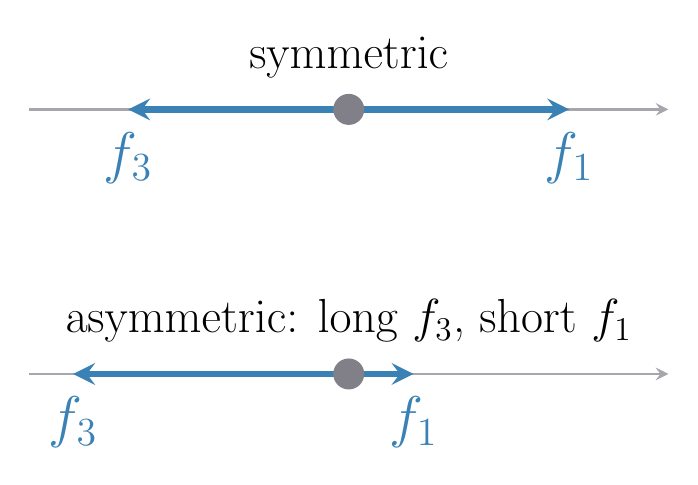
\begin{tikzpicture}[scale=2.8]
  \begin{scope}[shift={(0,1.2)}]
    \draw[axis] (-1.45,0) -- (1.45,0);
    \draw[feat] (0,0) -- (1,0);
    \draw[feat] (0,0) -- (-1,0);
    \node[pivotalBlue, below, lbl] at (1,-0.06)  {$f_1$};
    \node[pivotalBlue, below, lbl] at (-1,-0.06) {$f_3$};
    \fill[pivotalTaupe] (0,0) circle (2pt);
    \node[above, sm] at (0,0.1) {symmetric};
  \end{scope}
  \draw[axis] (-1.45,0) -- (1.45,0);
  \draw[feat] (0,0) -- (0.294,0);
  \draw[feat] (0,0) -- (-1.25,0);
  \node[pivotalBlue, below, lbl] at (0.294,-0.06)  {$f_1$};
  \node[pivotalBlue, below, lbl] at (-1.25,-0.06) {$f_3$};
  \fill[pivotalTaupe] (0,0) circle (2pt);
  \node[above, sm] at (0,0.1) {asymmetric: long $f_3$, short $f_1$};
\end{tikzpicture}
\end{document}
